\def\difficulty{2}
\sujet{Stochastic Geometry / Spatial Processes}
\index{Spatial Processes}
\begin{note}This tutorial aims to simulate different spatial point processes.\end{note}


\section{Poisson processes}
\index{Spatial Processes!Poisson Point Process}
This process simulates a conditional set of $point_{nb}$ points in a spatial domain $D$ defined by the values $x_{min}, x_{max}, y_{min}, 
y_{max}$.
In order to simulate a non conditional Poisson point process of intensity $\lambda$ within a domain $S$, it is necessary to generate a 
random number of points according to a Poisson law with the parameter $\lambda S$ : $point_{nb}=poisson(\lambda S)$ (i.e. the number of 
points is a random variable following a Poisson Law).

The coordinates of each point follow a uniform distribution.

\begin{figure}[htbp]
 \centering\caption{Conditional Poisson point process, with 200 points.}%
 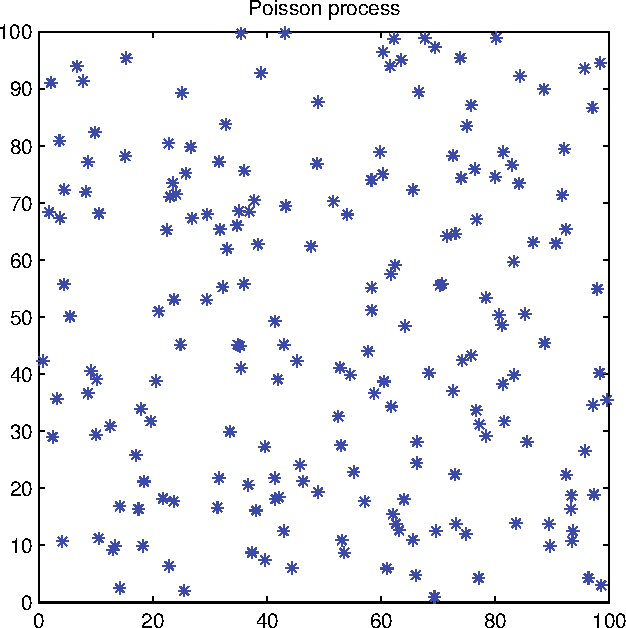
\includegraphics[width=7cm]{../matlab/poissonprocess}%
 \label{fig:spatialpp:enonce:ppp}%
\end{figure}

\begin{qbox}
\begin{enumerate}
	\item Simulate a conditional Poisson point process on a spatial domain $D$ with a fixed number of points (see Fig. 
\ref{fig:spatialpp:enonce:ppp}).
	\item Simulate a Gaussian distribution of points around a given center.
\end{enumerate}
\end{qbox}

\begin{mcomment}
\begin{mremark}
 The function \minline{poissrnd} can be used to generate and random variable following a Poisson law. Use \minline{rand} for generating uniform distribution random variables.
\end{mremark}
\end{mcomment}

\begin{pcomment}
\begin{premark}
Import \pinline{scipy.stats} to use the function \pinline{poisson} and \pinline{np.random} for more classical stochastic functions.
\end{premark}
\end{pcomment}


\section{Neyman-Scott processes}
\index{Spatial Processes!Neyman-Scott Point Process}
This process simulates aggregated sets of points within a spatial domain $D$ defined by the values $x_{min}, x_{max}, y_{min}, y_{max}$. 
For each aggregate ($n_{par}$), we first generate the random position of the 'parent' point. Then, the 'children' points are simulated in a 
neighborhood (within a square box of size $r_{child}^2$) of the 'parent' point. The number of points for each aggregate is either fixed or 
randomized according to a Poisson law of parameter $n_{child}$ (see Fig. \ref{fig:point_process_generation:neymanscott}).

\begin{figure}[htbp]
 \centering\caption{Neyman-Scott point process with $h_{child}=10$ and $n_{par}=10$}%
 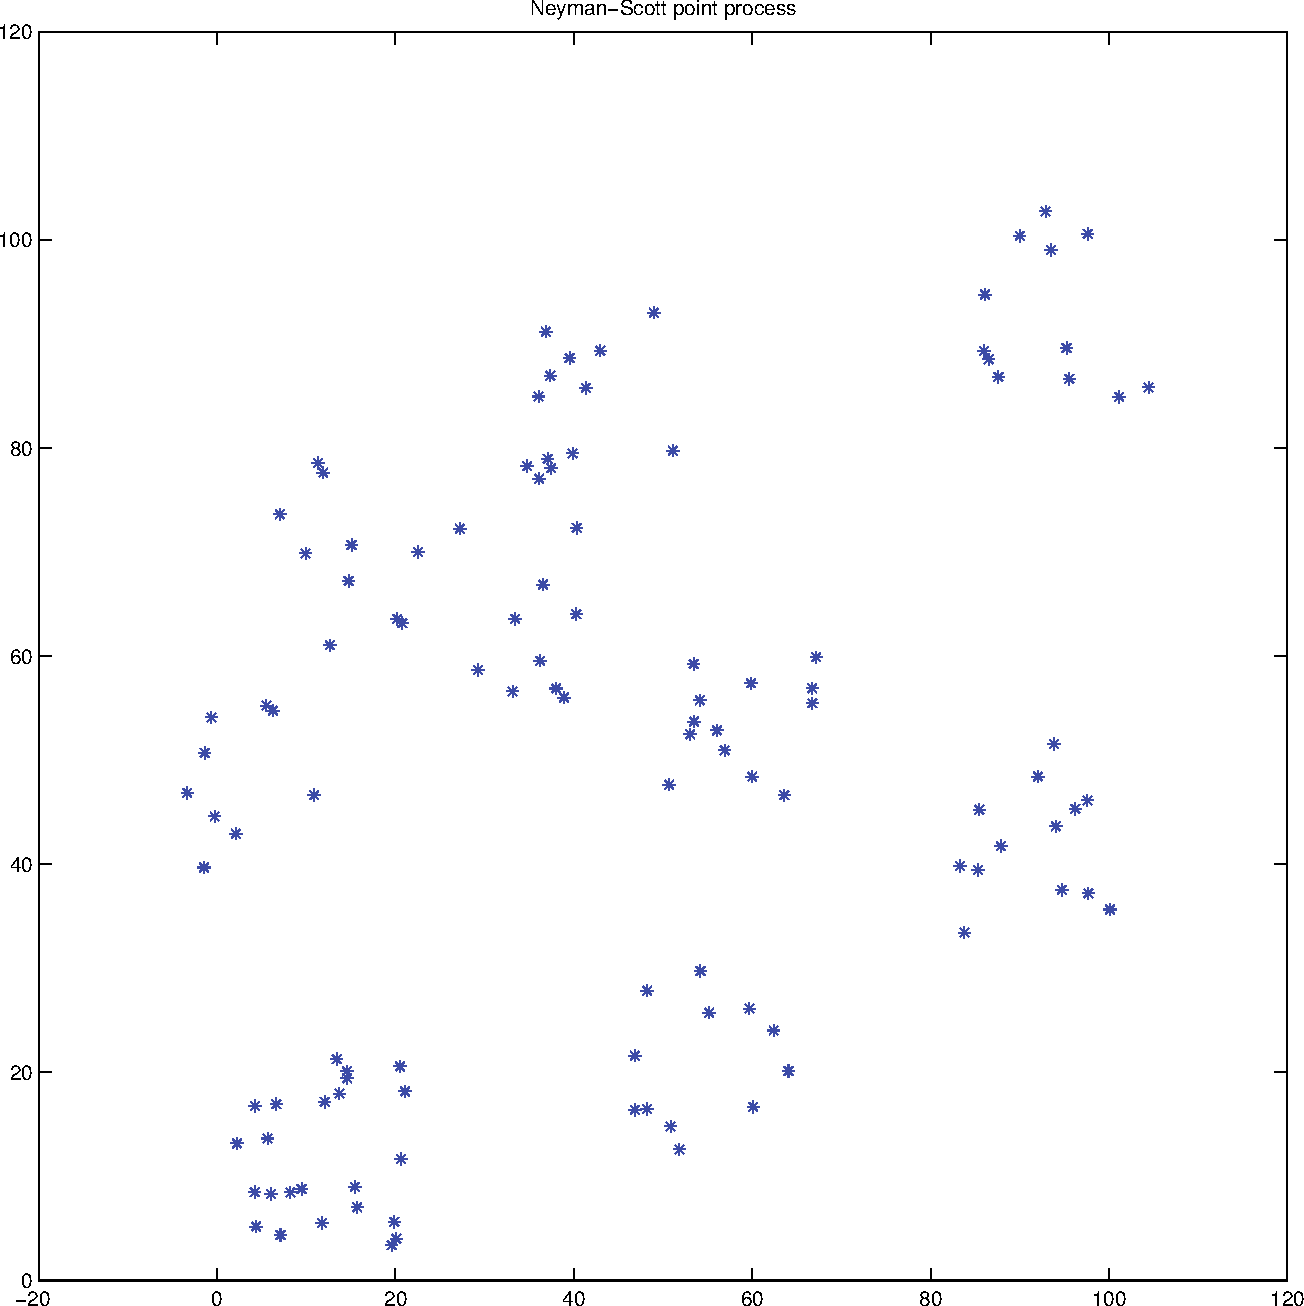
\includegraphics[width=8cm]{../matlab/neymanscottprocess}%
 \label{fig:point_process_generation:neymanscott}%
\end{figure}

\begin{qbox}
\begin{enumerate}
	\item Simulate a process of 3 aggregates with 10 points.
	\item Simulate a process of 10 aggregates with 5 points.
\end{enumerate}
\end{qbox}

\section{Gibbs processes}
\index{Spatial Processes!Gibbs Point Process}
The idea of Gibbs processes is to spatially distribute the points according to some laws of interactions (attraction or repulsion) within a 
variable range. 

Such a process can be defined by a cost function $f(d)$ that represents the cost associated to the presence of 2 separated points by a 
distance $d$ (see Fig. \ref{fig:point_process_generation:energyfunction}). For a fixed value $r$, if $f(d)$ is negative, there is a high 
probability to find 2 points 
at a distance $d$ (attraction). Conversely, if $f(d)$ is positive, there is a weak probability to find 2 points at a distance $d$ 
(repulsion).



\begin{itemize}
 \item Code such a function, with prototype \minline{function e=f(d)} or \pinline{def energy(d):}, where
 \[ f(d) = \left\{ 
  \begin{array}{l l}
    50 & \quad \text{if $0<d\leq 15$ }\\
    -10 & \quad \text{if $15<d\leq 30$}\\
    0 & \quad otherwise
  \end{array} \right.\]
\end{itemize}
\begin{figure}[htbp]
 \centering\caption{Energy function $f$.}%
 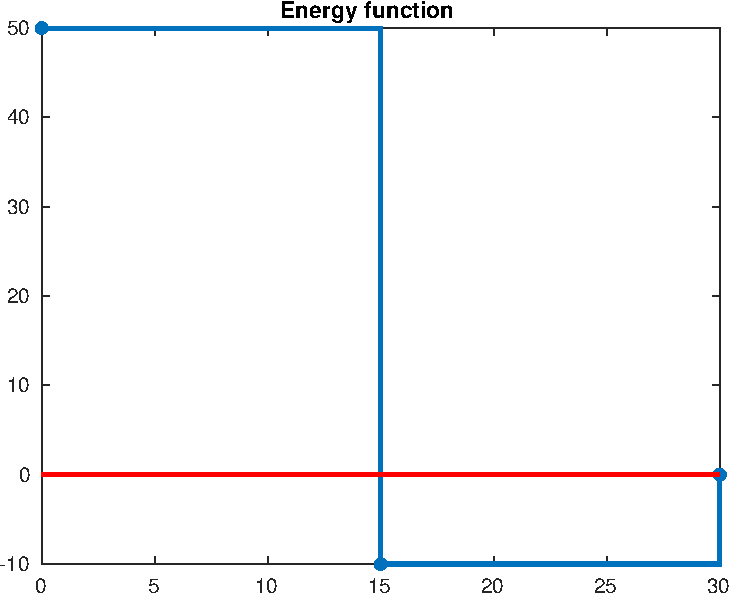
\includegraphics[width=6cm]{../matlab/energy.pdf}%
 \label{fig:point_process_generation:energyfunction}%
\end{figure}

%
The generation process reorganizes an initial Poisson point process within the spatial domain according to a specific cost piecewise 
constant function. The reorganization consists in a loop of $nb_{iter}$ iterations.
For each iteration, we calculate the total energy:
\begin{eqnarray}
e=\displaystyle\sum_{(i,j), i\neq j}f(dist(x_i,x_j))
\end{eqnarray}
The objective is to reduce this energy iteratively. At each  iteration step, we try to replace a point by four (for example) other random points and we 
calculate the energy for each new configuration. The initial point is either preserved or replaced (by one of the four points) according to the 
configuration of minimal energy (see Fig.\ref{fig:point_process_generation:enonce:gibbs}).
 
\begin{figure}[htbp]
 \centering\caption{Illustration of iterative construction of the Gibbs point process.}%
 \subfloat[Start with an initial distribution of points. The energy is computed for all pairs of points.]{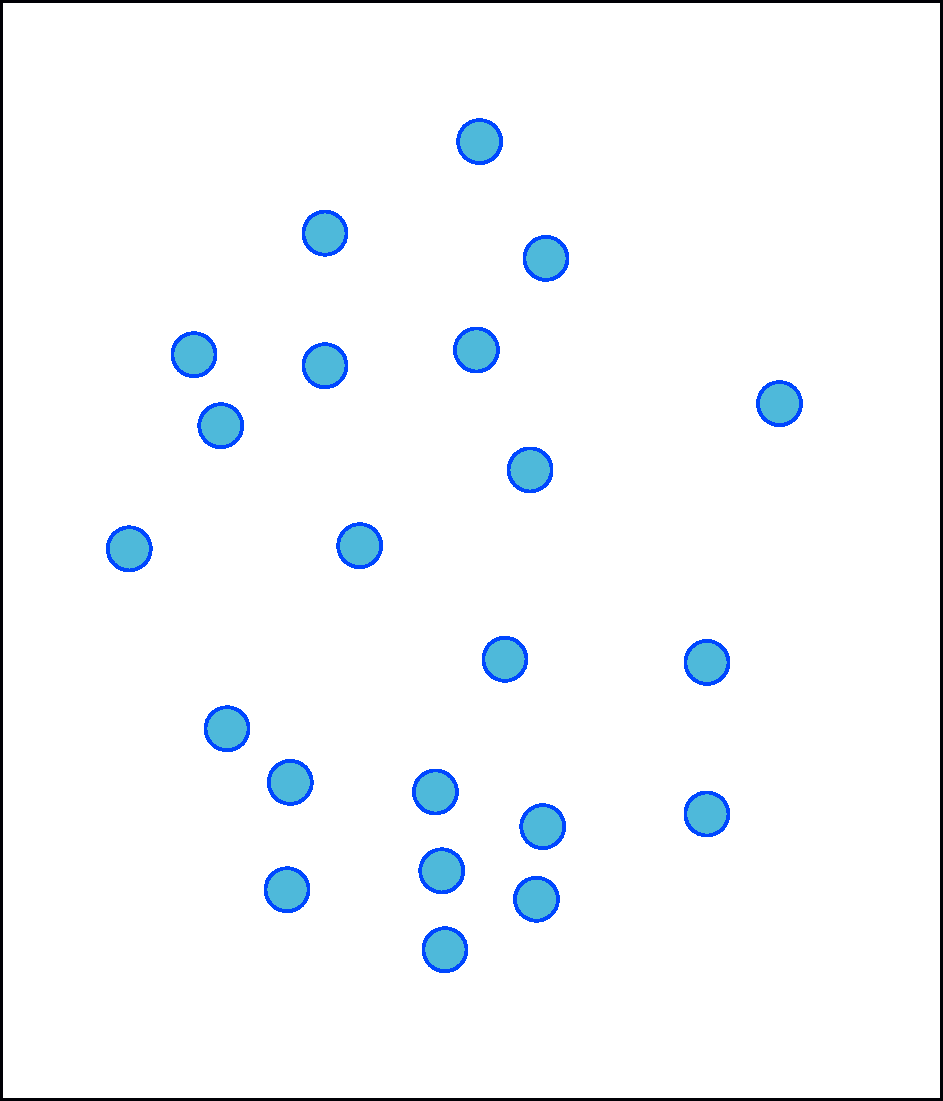
\includegraphics[width=.24\linewidth]{gibbs_0.pdf}}\hfill
 \subfloat[A random point is selected. ]{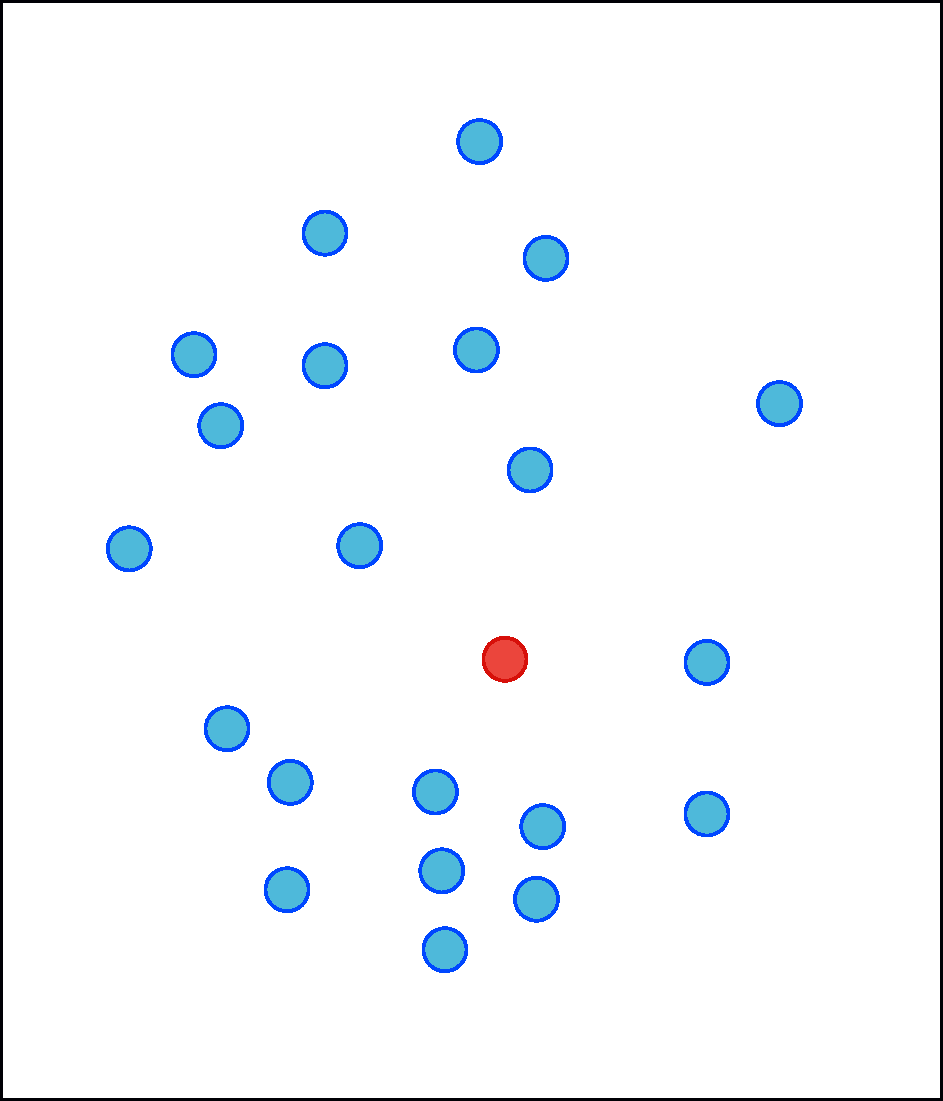
\includegraphics[width=.24\linewidth]{gibbs_1.pdf}}
 \hfill
 \subfloat[Four candidate points are randomly generated, the energy of these four new configurations is evaluated.]{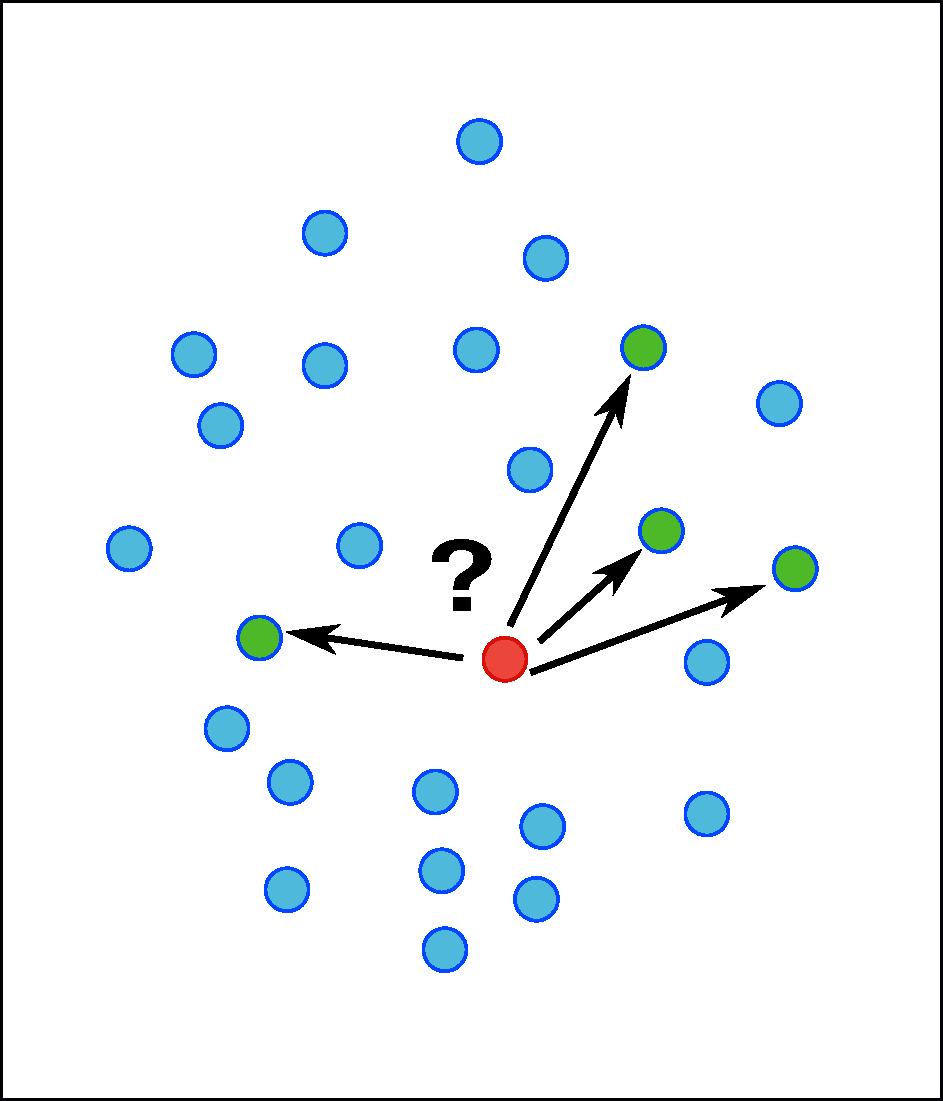
\includegraphics[width=.24\linewidth]{gibbs_2.pdf}}\hfill
 \subfloat[The configuration with the minimal energy is retained, other points are discarded.]{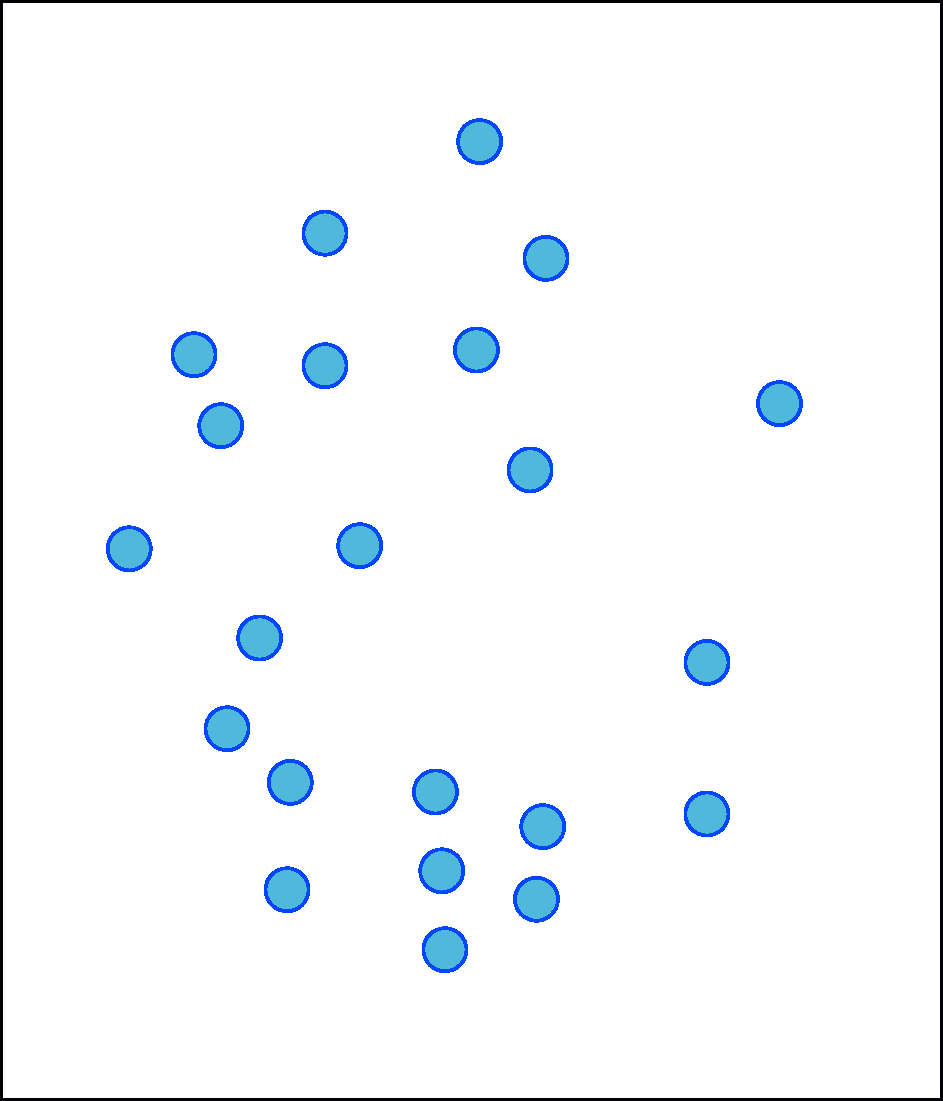
\includegraphics[width=.24\linewidth]{gibbs_3.pdf}}%
 \label{fig:point_process_generation:enonce:gibbs}%
\end{figure}


%
\begin{qbox}
\begin{enumerate}
        \item Code a function with the following prototype (the function \textit{energyFunction} is previously noticed $f$). It computes the energy between all the points present in an array of coordinates $[x, y]$ (the points that do not move) and point $[x_k,y_k]$ (the new point). The \textit{energyFunction} converts a distance to an 'energy', reflecting attractivity or repulsivity.
	\begin{mcomment}
\begin{matlab}
function e = energy(energyFunction, x, y, xk, yk)
\end{matlab}
\end{mcomment}

\begin{pcomment}
\begin{python}
def energy(P, eFunction=exampleEnergyFunction):
\end{python}
\end{pcomment}


	\item Simulate a regular point process by choosing a specific energy function.
	\item Change the cost function and simulate a few aggregated point processes (see Fig. \ref{fig:gibbsprocess}).
\end{enumerate}
\end{qbox}

\begin{pcomment}
 \begin{phelp}
Use the function \pinline{pdist} from \pinline{scipy.spatial.distance}, which computes pairwise distances of all points.  
 \end{phelp}
\end{pcomment}

\begin{mcomment}
 \begin{mhelp}
  Use the function \minline{pdist}, which computes pairwise distances of all points. You may also consider the \pinline{pdist2} function.
 \end{mhelp}

\end{mcomment}

\vspace*{-7pt}

\begin{figure}[H]
 \centering\caption{Gibbs agregated point process and its energy function.}%
 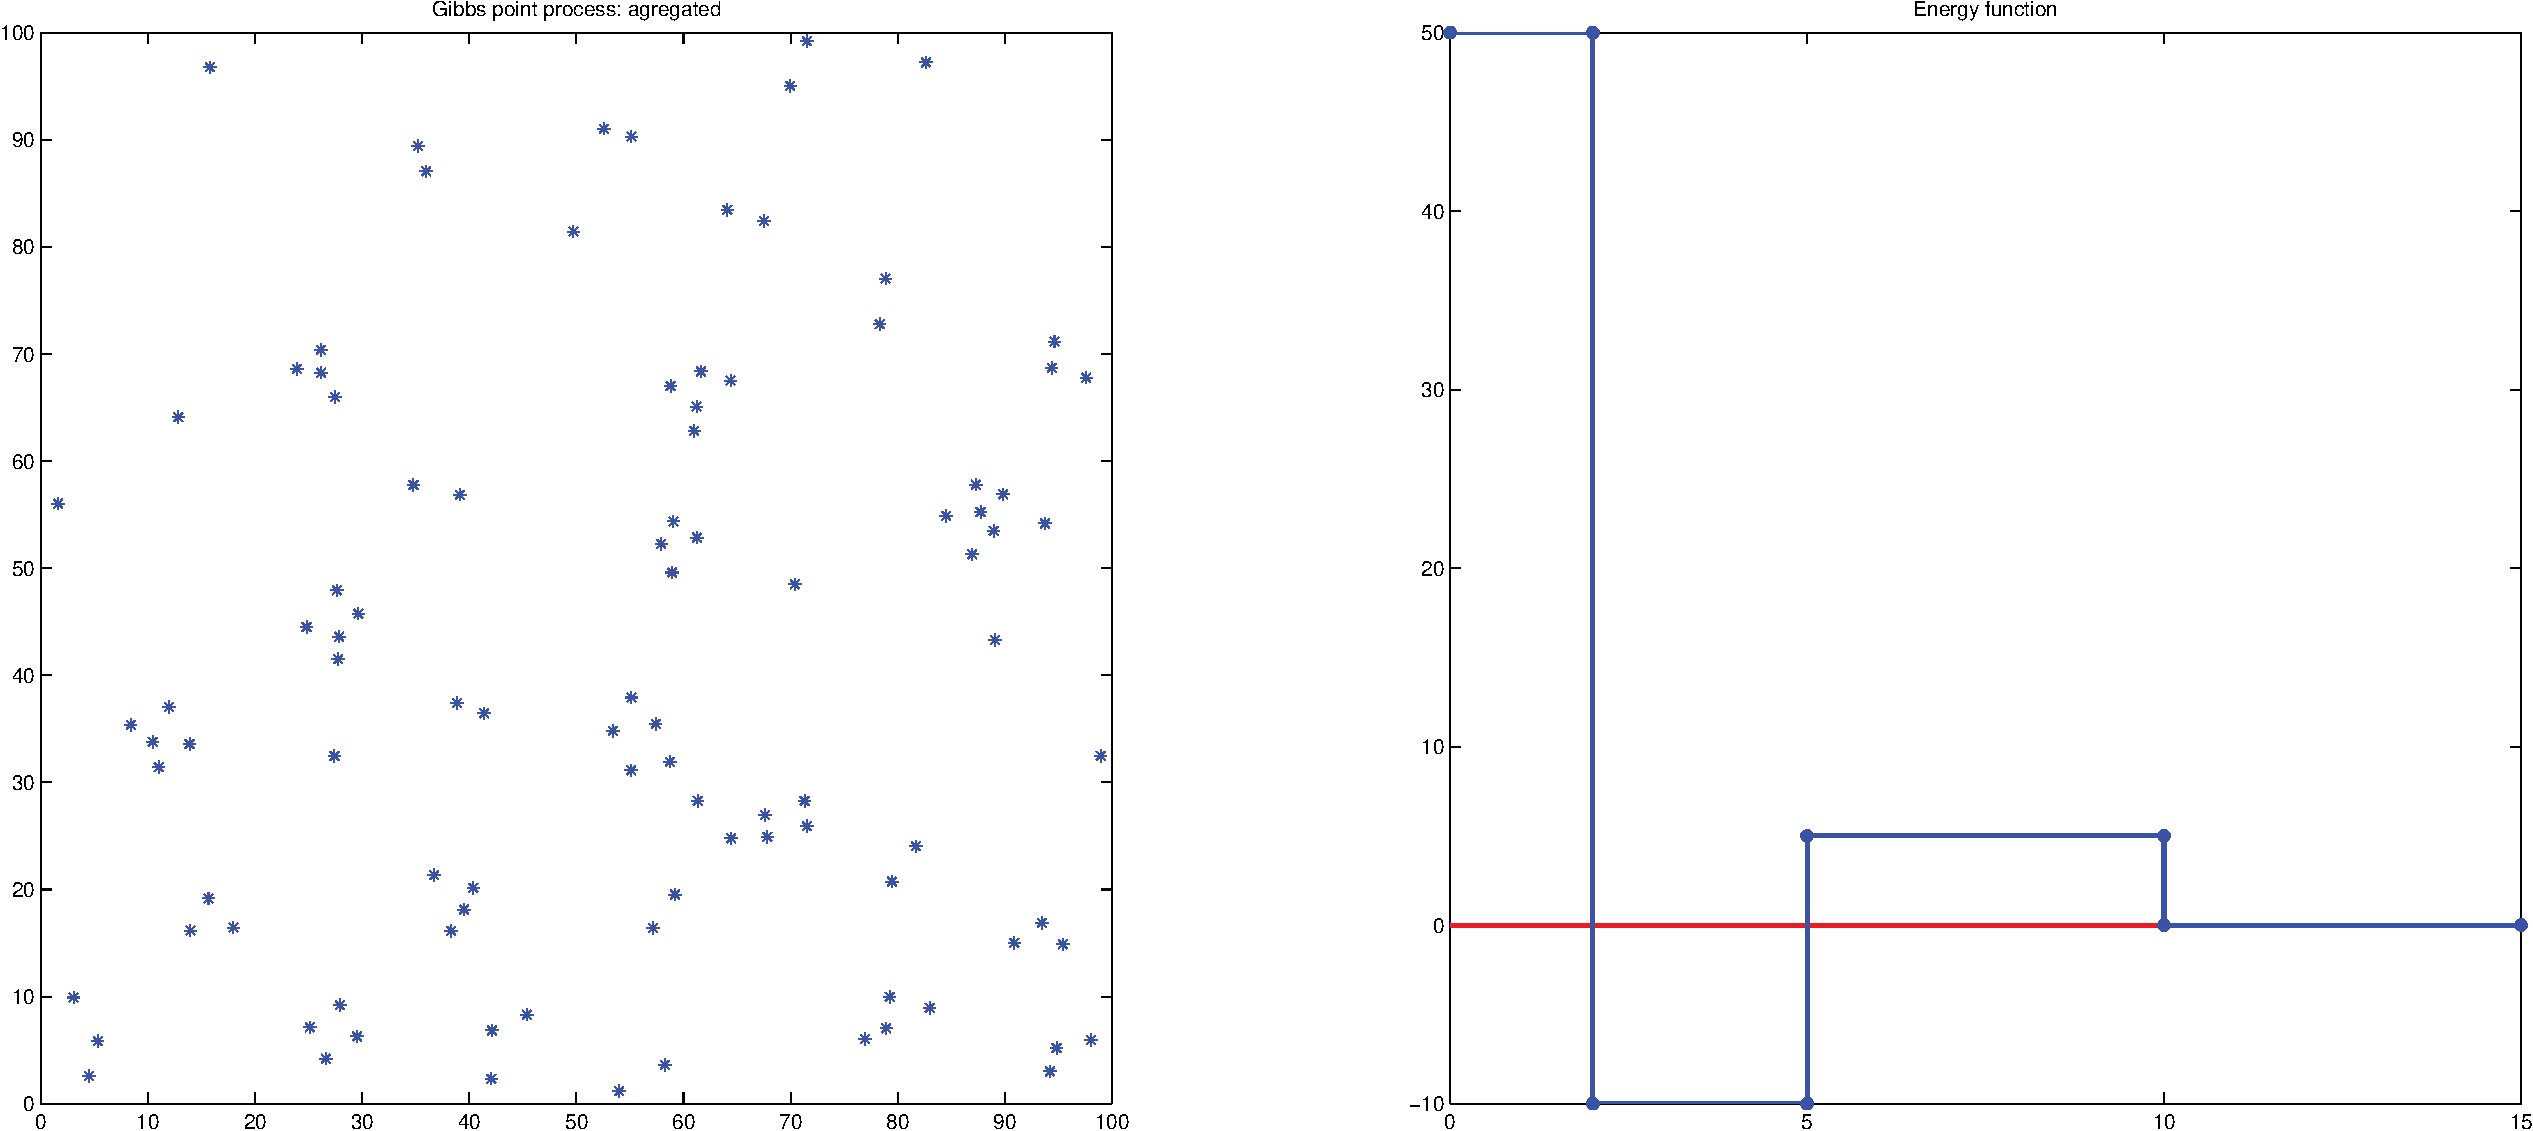
\includegraphics[width=0.8\textwidth]{../matlab/gibbsprocess-crop.pdf}%
 \label{fig:gibbsprocess}%
\end{figure}

\vspace*{-10pt}

\section{Ripley function}\vspace*{-3pt}
\index{Spatial Processes!Ripley Functions}\index{Spatial Processes!Characterization}
The Ripley function $K(r)$ characterizes the spatial distribution of the points.
For a Poisson process of density $\lambda$, $\lambda K(r)$ is equal to the mean value of the number of neighbors at a distance lower than 
$r$ to any point. In the case where the process is not known ($\lambda$?), the Ripley function has to be estimated (approximated) with the 
unique known realization. It is the first estimator of $K(r)$:
\begin{eqnarray}
K(r)=\frac{1}{\lambda}\frac{1}{N}\sum_{i=1}^N\sum_{i\neq j}k_{ij}
\end{eqnarray}
where $N$ is the number of points in the studied domain $D$, $\lambda=N/D$ is the estimator of the density of the process and $k_{ij}$ takes 
the value $1$ if the distance between the point $i$ and the point $j$ is lower than $r$, and $0$ in the other case.

We denote:
\begin{eqnarray}
 L(r) = \sqrt{K(r)/\pi}
\end{eqnarray}

\begin{qbox}
\begin{enumerate}
	\item Code a function to compute K (\lstinline!function K=ripley(points, box, r)!), with \lstinline!points! being the considered 
points, \lstinline!box! the simulation domain, and $r$ the distance (or an array of all distances). 
	\item Calculate the Ripley function for an aggregated point process, a Poisson point process and a regular point process.
	\item Display the value $L(r)-r$ as in Fig \ref{fig:point_process_generation:ripleyL}.
\end{enumerate}
\end{qbox}

\vspace*{-7pt}

\begin{figure}[H]
 \centering\caption{Ripley's function $L(r)-r$.}%
 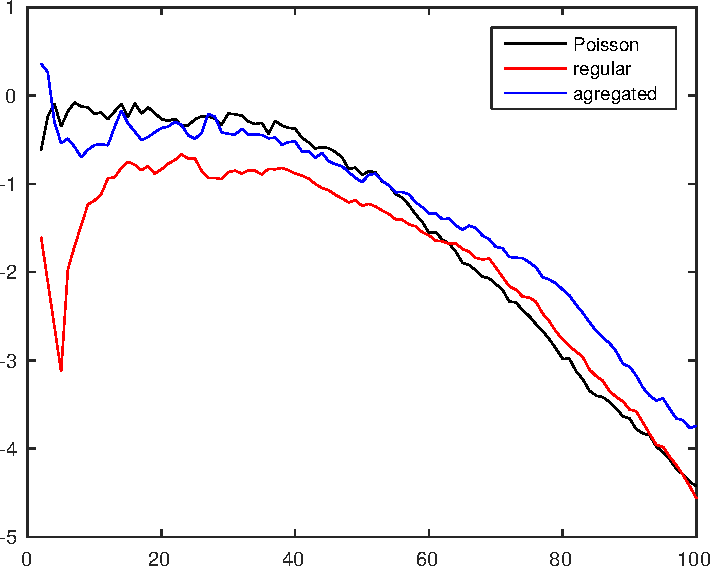
\includegraphics[width=5.5cm]{../matlab/ripley.pdf}%
 \label{fig:point_process_generation:ripleyL}%
\end{figure}

\vspace*{-7pt}

\section{Marked point processes}\vspace*{-5pt}
\index{Spatial Processes!Marked Process}
To simulate a complex point process, it can be useful to associate several random variables (marks) for each point.

\begin{qbox}
\begin{enumerate}
	\item Simulate a disk process, where the points (disk centers) are defined according to a Poisson process and the radii are selected 
with a Gaussian law.
	\item Add a second mark for allocating a color to each disk (uniform law).
\end{enumerate}
\end{qbox}%\enlargethispage{2cm}

An example result is shown in Fig. \ref{fig:point_process_generation:circles}
\vspace*{-10pt}
\begin{figure}[H]
 \centering\caption{A Poisson point process is used to generates the center of the circles. The radii are chosen according a Gaussian law, and the 
 	color according a uniform law.}%
 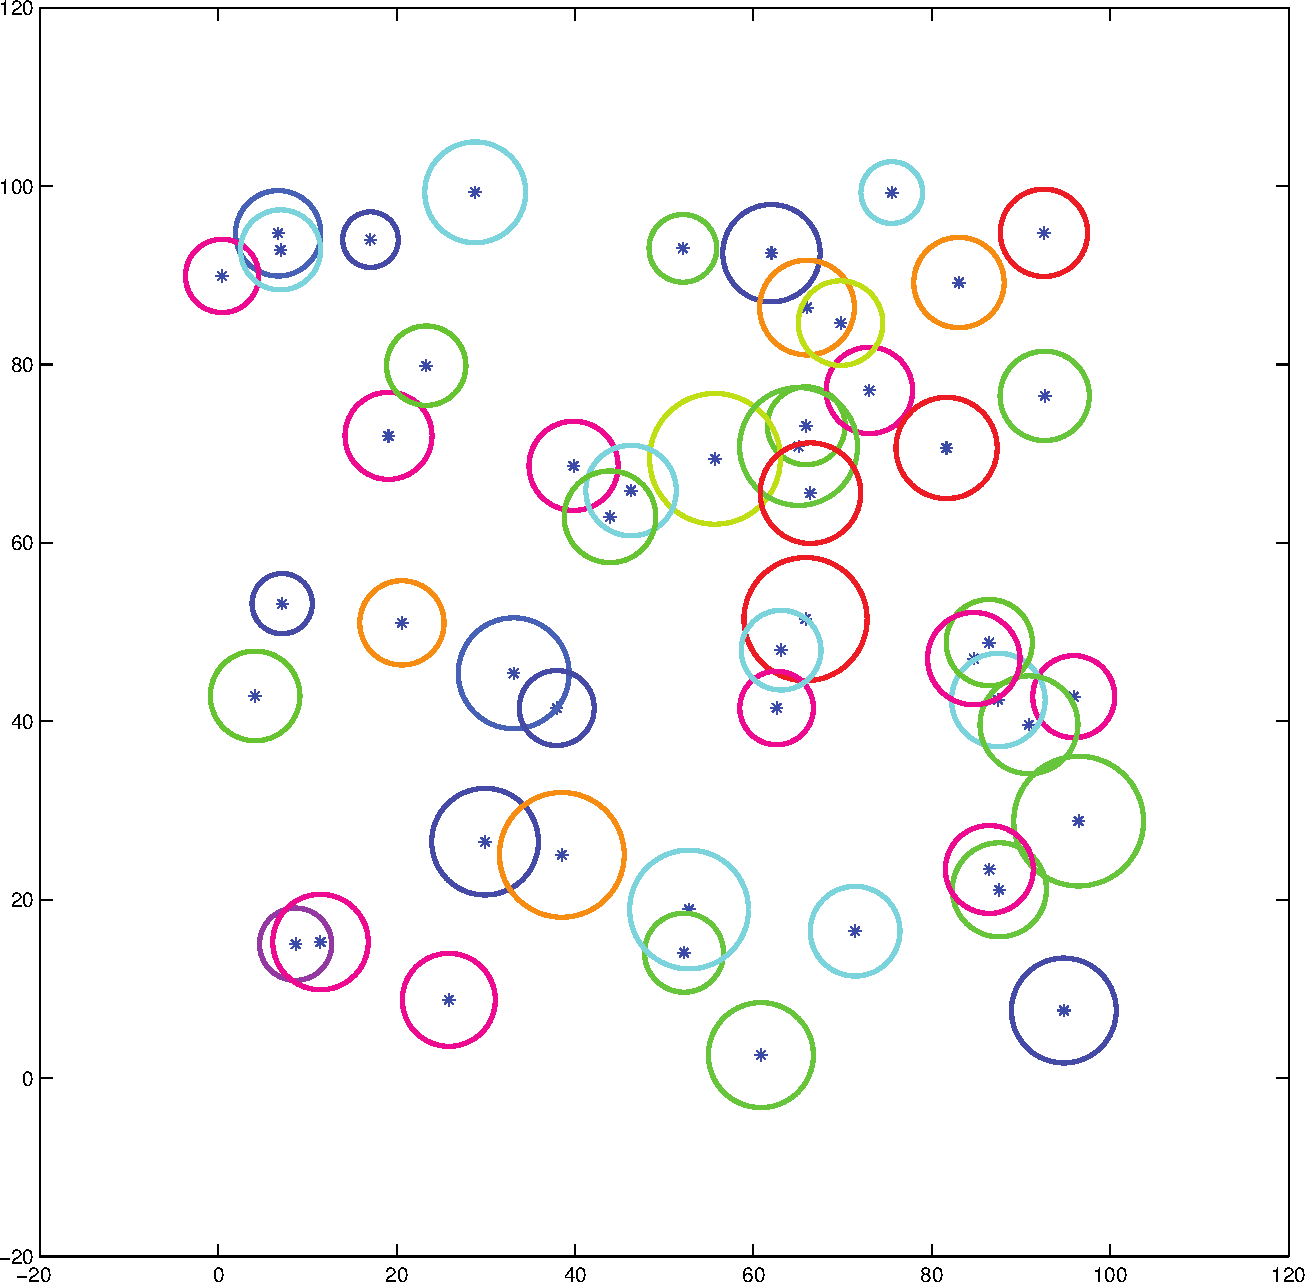
\includegraphics[width=5.5cm]{../matlab/circles.pdf}%
 \label{fig:point_process_generation:circles}%
\end{figure}

